\begin{scanpage}{0162}{144}
\begin{minipage}[t]{.46\linewidth}\vspace{0pt}\centering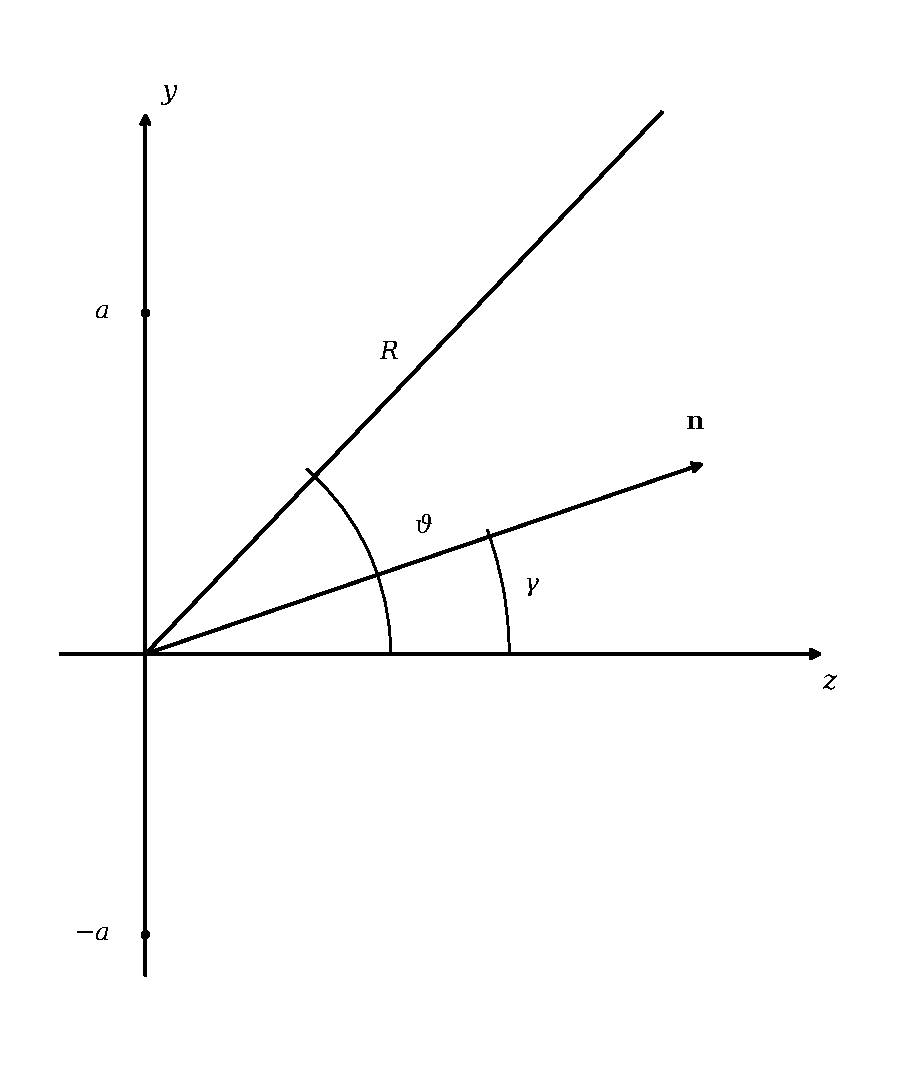
\includegraphics[width=.8\linewidth]{images/recreated/c-0162-fig63.pdf}\par\raggedright
Figure 63. The cross section of a disk with the plane yoz; $\mathbf n$ is the normal to the incident wave front.
\end{minipage}\hfill
\begin{minipage}[t]{.46\linewidth}\vspace{0pt}\centering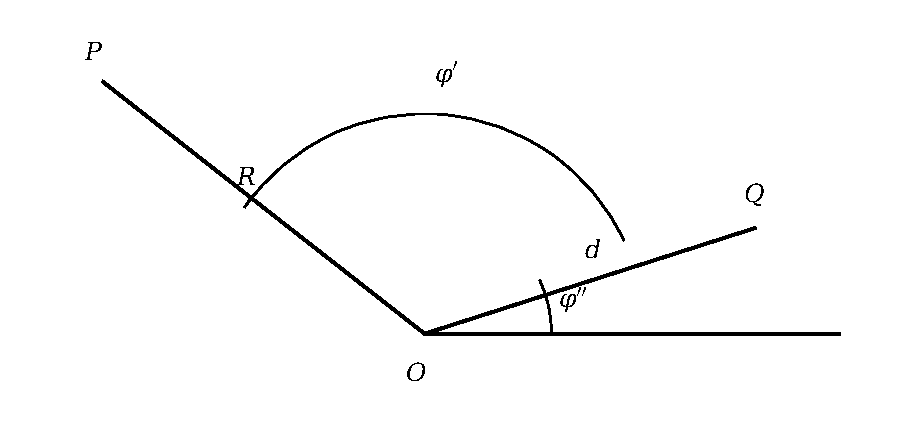
\includegraphics[width=\linewidth]{images/recreated/c-0162-fig64.pdf}\par\raggedright
Figure 64. Excitation of a half-plane by an elementary dipole which is located at the point Q.
\end{minipage}
\par\bigskip
Let us compare the shading of spherical and cylindrical waves by a half-plane. Let an ideally conducting half-plane be found in free space, and let there be an elementary dipole at the point Q (Figure 64). Let us find the field in the plane perpendicular to the half-plane's edge and passing through the point Q.

In accordance with the reciprocity principle, it is determined for the electric dipole by the relationship
\[
E_z=\frac{p_z}{p_{0z}}E_z(Q),\tag{24.08}
\]
and for the magnetic dipole by the relationship
\[
H_z=\frac{m_z}{m_{0z}}H_z(Q).\tag{24.09}
\]
Here $p_z$ ($m_z$) is the electric (magnetic) dipole moment found at the point Q; $p_{0z}$ and $m_{0z}$ are the moments of the auxiliary dipoles which are placed at the point P; $E_z(Q)$ and $H_z(Q)$ are the fields created by the auxiliary dipoles at the point Q.
\end{scanpage}
